% Springer CCIS / LNCS format -- SPELLL 2026 double-blind submission.
% Derived from ccis_template.tex (LLNCS macro package, v2.21 of 2022/01/12).
\documentclass[runningheads]{llncs}
%
\usepackage[T1]{fontenc}
% Without this, T1 encoding falls back to the EC bitmap (Type 3) fonts, which
% render heavy and smeared at small sizes and which Springer does not want.
% Latin Modern is a vector redrawing of Computer Modern, so the look is
% unchanged.
\usepackage{lmodern}
% T1 fonts will be used to generate the final print and online PDFs,
% so please use T1 fonts in your manuscript whenever possible.
%
\usepackage{amsmath,amssymb,amsfonts}
\usepackage{graphicx}
\usepackage{textcomp}
\usepackage{color}
\usepackage{booktabs}
\usepackage{multirow}
\usepackage{array}
\usepackage{tikz}
\usetikzlibrary{arrows.meta,positioning}
\usepackage{hyperref}

% Pipeline-diagram palette, matching the pastel fills of the original figure.
\definecolor{pipegreen}{rgb}{0.78,0.94,0.80}
\definecolor{pipeblue}{rgb}{0.80,0.87,0.97}
\definecolor{pipepink}{rgb}{0.95,0.81,0.95}
\definecolor{pipeyellow}{rgb}{0.98,0.96,0.76}
\definecolor{pipeorange}{rgb}{0.99,0.85,0.73}
\definecolor{pipegray}{rgb}{0.90,0.90,0.90}

% Diagram labels are typeset by LaTeX so they carry the body text font.
\tikzset{
  blk/.style={
    rounded corners=2pt, draw=black!45, line width=0.3pt,
    align=center, inner sep=2pt, minimum height=6.5mm, font=\scriptsize
  },
  flow/.style={draw=black!55, line width=0.3pt},
  arw/.style={flow, -{Stealth[length=1.2mm,width=1mm]}}
}
\renewcommand\UrlFont{\color{blue}\rmfamily}
\urlstyle{rm}
\hypersetup{
  hidelinks,
  pdfauthor={},
  pdfsubject={},
  pdfkeywords={}
}

% Custom column type for tables
\newcolumntype{L}[1]{>{\raggedright\arraybackslash}p{#1}}

% Single-column LNCS measure is narrower than the IEEE two-column one; allow
% the line breaker extra slack rather than leaving overfull boxes.
\emergencystretch=2em

% The split-panel figures are taller than LaTeX's default \topfraction (0.7)
% allows, which strands them past the bibliography. Loosen the float rules.
\renewcommand{\topfraction}{0.9}
\renewcommand{\bottomfraction}{0.8}
\renewcommand{\textfraction}{0.07}
\renewcommand{\floatpagefraction}{0.75}

\begin{document}
%
\title{Robust Speaker-Independent Vocal Pathology Detection through Integrated Acoustic and Nonlinear Dynamics on the German Saarbr\"ucken Voice Database}
%
\titlerunning{Robust Speaker-Independent Vocal Pathology Detection}
%
% Double-blind submission: author names, affiliations and e-mail addresses are
% withheld in accordance with the SPELLL 2026 review policy.
\author{Anonymous Author(s)}
%
\authorrunning{Anonymous Author(s)}
%
\institute{Affiliation withheld for double-blind review}
%
\maketitle              % typeset the header of the contribution
%
\begin{abstract}
Voice pathology classification is difficult because pathological speech is nonlinear and varies across time scales, and traditional acoustic metrics describe only part of that behaviour. This paper presents a method for both binary (healthy/pathological) and multi-class (neurological/structural disease group) classification of vocal pathology. It combines multifractal features extracted with Multifractal Detrended Fluctuation Analysis (MFDFA) and standardised acoustic features from the extended Geneva Minimalistic Acoustic Parameter Set (eGeMAPS). Experiments on the Saarbrücken Voice Database use strict speaker-independent cross-validation to rule out speaker-level leakage, a control that much of the earlier literature omits. Healthy speakers in this corpus are much younger than pathological ones (mean age 27.1 vs.\ 54.0 years), so every result is reported with and without age and sex as inputs, next to age-only and sex-only baselines and an evaluation on age- and sex-matched subsets. Under five-fold speaker-independent cross-validation, binary pathology detection reaches a macro F1 of 0.882 with age and sex included, but age alone reaches 0.830. Without demographic inputs the acoustic and nonlinear features reach 0.760, and 0.679 on the matched subset. Disease-group classification reaches 0.635 without demographic inputs and 0.575 on matched data. The MFDFA descriptors alone reach 0.644 on the binary task but add no measurable gain over eGeMAPS.

\keywords{Voice Pathology Detection \and Multifractal Analysis \and Fractal
Dimension \and MF-DFA \and Saarbr\"ucken Voice Database \and Nonlinear Speech
Analysis.}
\end{abstract}
%
%
%
  %--------------------------------------------------------------
  \section{Introduction}
  \label{sec:introduction}
  %--------------------------------------------------------------

Voice disorders are common. They arise from structural pathology of the vocal folds, from neurogenic disorders of motor coordination, and from functional or psychogenic causes. Diagnosis normally combines instrumental procedures such as laryngoscopy with perceptual evaluation by a clinician. That combination is accurate, but perceptual judgement is subjective and demands considerable clinical expertise.

Automatic detection is attractive precisely because it removes that subjectivity. Most systems for recognising pathological voices rely on standard spectral parameters such as MFCCs and F0. These describe the spectral properties of speech well, but they capture little of the temporal and nonlinear behaviour typical of pathological voices.

Speech production is a nonlinear process in which airstream initiation, vocal fold vibration, and articulation all interact. In pathological voices these dynamics can become unstable. Fractal and multifractal theory offers a way to quantify that instability.

This work applies multifractal detrended fluctuation analysis to speech recordings from speakers with diagnosed disorders. Multifractal analysis describes a time series through its scaling properties across time scales. A monofractal signal is characterised by a single scaling exponent; a multifractal one needs a spectrum of local exponents, obtained by varying the moment order $q$ of the analysis.

The question addressed here is whether the multifractal descriptors obtained through MFDFA help detect voice pathology, either on their own or alongside standard acoustic parameters.

  This work differs from earlier fractal-based voice pathology studies in four ways. First, we use the full multifractal spectrum from MFDFA rather than a single scalar fractal dimension, which gives scaling information across several moment orders. Second, one pipeline handles both binary (healthy vs.\ pathological) and multi-class (neurological vs.\ structural) classification, where most earlier studies treat only binary detection. Third, cross-validation is strictly speaker-independent (\texttt{StratifiedGroupKFold}), so recordings from one speaker never appear in both the training and the test split. This guards against the data leakage known to produce optimistic results in much of the earlier literature \cite{saenzlechon2006}. Fourth, because age alone separates healthy from pathological speakers in this corpus, every result is reported with and without age and sex, and on age- and sex-matched subsets. A feature ablation study then quantifies what MFDFA contributes alone and in combination for each classification task.

  %--------------------------------------------------------------
  \section{Related Work}
  \label{sec:related_work}
  %--------------------------------------------------------------

  Automatic detection of voice pathologies has traditionally relied on acoustic features such as MFCCs, perturbation measures, and spectral statistics combined with statistical or machine learning classifiers \cite{godino2006,alnasheri2017,rai2025}. Standardised clinical frameworks have further formalised multi-parameter acoustic assessment: the Dysphonia Severity Index (DSI) combines jitter, phonation time, and intensity into a perceptually anchored score \cite{wuyts2000}, while standardised assessment protocols specify perturbation and noise measures as a clinical evaluation battery \cite{dejonckere2001}. Although these spectral and perturbation-based descriptors capture important phonatory characteristics, they are inherently linear and cannot represent the nonlinear or multi-scale temporal irregularities often present in pathological voices.

  Nonlinear analysis methods have therefore also been explored for pathological speech. Little et al.\ demonstrated that recurrence quantification analysis and fractal scaling properties extracted from sustained phonations can complement conventional acoustic measures for voice disorder detection, achieving correct classification performance above 91\% \cite{little2007b}. Nonlinear dynamical measures such as correlation dimension, Lyapunov exponents, and entropy statistics have been applied to separate healthy from pathological voices with high accuracy on clinical voice databases \cite{henriquez2009,little2007}. Temporal complexity measures therefore carry information that standard spectral descriptors miss. Recurrence plot-based characterisation has also been applied to specific vocal fold pathologies including hyperfunctional dysphonia, laryngitis, and vocal fold polyp, achieving classification accuracy above 90\% on the Saarbrücken Voice Database \cite{krishnan2026}.

  Beyond binary detection, recent work has addressed multi-class voice disorder classification. Orozco-Arroyave et al.\ found that different feature families are required to capture the distinct acoustic signatures of neurological, functional, and laryngeal disorders \cite{orozco2015}. Fractal dimension in multiresolution frameworks has also achieved detection rates above 90\% via per-subband power-spectrum analysis \cite{ali2016,kumar2014}.

  Multifractal detrended fluctuation analysis (MFDFA) extends scalar fractal characterisation by modelling scaling behaviour across multiple moments and time scales \cite{mfdfa}. Multifractal methods have proven effective in other biomedical domains, most notably in demonstrating the multifractal structure of healthy versus diseased heartbeat dynamics \cite{ivanov1999}. Closer to the present work, multifractal analysis has been applied directly to speech signals for glottal activity detection, which shows that the method can capture nonlinear phonatory dynamics \cite{lal2020multifractal}. Speech-based disease detection has also benefited from careful acoustic feature design: Tsanas et al.\ developed 132 dysphonia measures from sustained vowels for high-accuracy Parkinson's disease classification, and showed that engineered descriptors can match or exceed purely data-driven methods in clinical tasks \cite{tsanas2012}. Sai Jahnavi et al.\ likewise detected Parkinson's disease from speech alone using excitation source, voice quality, and prosodic features from sustained vowels \cite{jahnavi2020}. MFDFA applied to voice pathology detection, and particularly to multi-class classification, remains comparatively underexplored.

  One methodological concern cuts across all of this work: speaker-level data leakage. Sáenz-Lechón et al.\ found that systems evaluated without controlling for speaker identity yield optimistic estimates that fail to generalise to unseen speakers, and recommended speaker-independent cross-validation as standard practice \cite{saenzlechon2006}.


  %--------------------------------------------------------------
  \section{Dataset Description}
  \label{sec:dataset}
  %--------------------------------------------------------------

  The experiments in this study use recordings from the Saarbrücken Voice Database (SVD)~\cite{svd}, a widely used clinical corpus of healthy and pathological voices. The original audio is stored in the proprietary \texttt{.nsp} format and is converted to standard \texttt{.wav} for preprocessing and feature extraction. SVD contains several vowels and connected-speech recordings, but this work uses only the sustained vowel \textit{/a/} at normal pitch (\texttt{a\_n}), which gives a stable phonation condition for cross-speaker comparison.

  Table~\ref{tab:dataset_stats} summarises the dataset used in the experiments.

  \begin{table}[htbp]
  \centering
  \caption{Dataset Statistics}
  \label{tab:dataset_stats}
  \begin{tabular}{ll}
  \toprule
  \textbf{Statistic} & \textbf{Value} \\
  \midrule
  Total recordings (all tokens) & 23,119 \\
  Unique speakers & 1,355 \\
  Pathology classes & 12 (+ healthy) \\
  Samples for token (\texttt{a\_n}) & 1,656 \\
  Sex distribution & 65\% female, 35\% male \\
  Mean age, healthy / pathological\textsuperscript{a} & 27.1 / 54.0 years \\
  \bottomrule
  \multicolumn{2}{l}{\scriptsize \textsuperscript{a}In the classification set of Section~\ref{sec:pipeline}.}
  \end{tabular}
  \end{table}

  The \texttt{a\_n} subset is class-imbalanced, as clinical speech datasets usually are. Pathology classes with too few speakers for reliable speaker-independent cross-validation are excluded. Parkinson's disease has a single \texttt{a\_n} recording and hypotonic dysphonia five, so neither is analysed on its own. The nine disorders retained span neurological, structural, and functional aetiologies: recurrent laryngeal nerve paralysis (breathiness from vocal fold immobility); spasmodic dysphonia (involuntary voice breaks from laryngeal dystonia); vocal fold nodules (hoarseness from bilateral overuse lesions); vocal fold polyp (breathiness from asymmetric fold vibration); Reinke's edema (a lowered, hoarse voice from swelling of the vocal fold cover); laryngitis (hoarseness from laryngeal mucosal inflammation); hyperfunctional dysphonia (strained voice from excessive laryngeal tension); psychogenic dysphonia (voice disorder of psychological aetiology without organic pathology); and functional dysphonia (dysphonia from maladaptive laryngeal behaviour without an identifiable organic cause).

  The classes also differ in age. In the classification set (Section~\ref{sec:pipeline}), healthy speakers are $27.1 \pm 10.9$ years old on average and pathological speakers $54.0 \pm 15.0$ (Mann--Whitney $p < 10^{-100}$). SVD's healthy group consists mostly of young adults: of its 687 healthy \texttt{a\_n} recordings, 100 come from speakers over 40 and 25 from speakers over 60. A classifier trained on this corpus can therefore exploit age, either directly or through age-related changes in the voice, and Section~\ref{sec:experiments} controls for this.

  \begin{figure}[htbp]
  \centering
  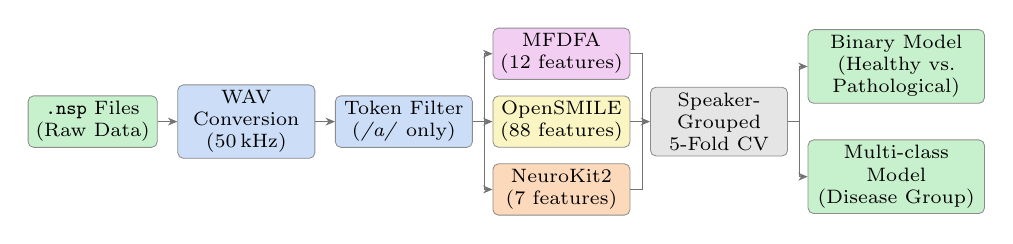
\begin{tikzpicture}
    % Preprocessing chain, left to right.
    \node[blk, fill=pipegreen, text width=15mm] (raw) {\texttt{.nsp} Files\\(Raw Data)};
    \node[blk, fill=pipeblue, text width=16mm, right=2.5mm of raw] (wav)
      {WAV Conversion\\(50\,kHz)};
    \node[blk, fill=pipeblue, text width=16mm, right=2.5mm of wav] (tok)
      {Token Filter\\(\textit{/a/} only)};

    % Feature families, stacked in a single column.
    \node[blk, fill=pipeyellow, text width=16mm, right=2.5mm of tok] (os)
      {OpenSMILE\\(88 features)};
    \node[blk, fill=pipepink, text width=16mm, above=2mm of os] (mf)
      {MFDFA\\(12 features)};
    \node[blk, fill=pipeorange, text width=16mm, below=2mm of os] (nk)
      {NeuroKit2\\(7 features)};

    % Speaker-grouped cross-validation.
    \node[blk, fill=pipegray, text width=16mm, right=2.5mm of os] (cv)
      {Speaker-Grouped\\5-Fold CV};

    % The two classification tasks.
    \node[blk, fill=pipegreen, text width=21mm, right=2.5mm of cv, yshift=7mm]
      (bin) {Binary Model\\(Healthy vs.\\Pathological)};
    \node[blk, fill=pipegreen, text width=21mm, right=2.5mm of cv, yshift=-7mm]
      (mc) {Multi-class Model\\(Disease Group)};

    \draw[arw] (raw) -- (wav);
    \draw[arw] (wav) -- (tok);

    % Fan out to the feature extractors.
    \coordinate (fanout) at ([xshift=1.5mm]tok.east);
    \draw[flow] (tok.east) -- (fanout);
    \draw[arw] (fanout) |- (mf.west);
    \draw[arw] (fanout) -- (os.west);
    \draw[arw] (fanout) |- (nk.west);

    % Merge the feature tables.
    \coordinate (fanin) at ([xshift=1.5mm]os.east);
    \draw[flow] (mf.east) -| (fanin);
    \draw[flow] (nk.east) -| (fanin);
    \draw[flow] (os.east) -- (fanin);
    \draw[arw] (fanin) -- (cv.west);

    % Fan out to the two tasks.
    \coordinate (split) at ([xshift=1.5mm]cv.east);
    \draw[flow] (cv.east) -- (split);
    \draw[arw] (split) |- (bin.west);
    \draw[arw] (split) |- (mc.west);
  \end{tikzpicture}
  \caption{Overview of the preprocessing and feature extraction pipeline. Raw NSP recordings are converted to WAV format, metadata manifests are generated, and sustained vowel tokens are selected. Multiple feature families are then extracted and merged before training classification models using speaker-grouped cross-validation.}
  \label{fig:data_pipeline}
  \end{figure}

  %--------------------------------------------------------------
  \section{Feature Extraction}
  \label{sec:features}
  %--------------------------------------------------------------

  Each recording is decoded to mono at its native 50\,kHz sampling rate and amplitude-normalised before any feature is computed. Three signal-derived families are then extracted, giving 107 features in total: 12 multifractal descriptors, 88 standardised paralinguistic parameters, and 7 nonlinear complexity measures. Two speaker metadata variables are appended to these.

  \subsection{Multifractal Features}

  Multifractal detrended fluctuation analysis quantifies how the fluctuations of a signal scale with the size of the window over which they are measured, and how that scaling changes when large and small fluctuations are weighted differently~\cite{mfdfa}. For a recording $x(k)$ of length $N$, the analysis starts from the cumulative profile
  \begin{equation}
  Y(i) = \sum_{k=1}^{i} \left[ x(k) - \bar{x} \right], \qquad i = 1,\dots,N ,
  \end{equation}
  which is divided into non-overlapping windows of length $s$ from both ends of the series. A polynomial of order $m$ is fitted within each window $v$ and removed, leaving the local variance $F^2(v,s)$. Averaging these variances with moment order $q$ gives the fluctuation function
  \begin{equation}
  F_q(s) = \left\{ \frac{1}{2N_s} \sum_{v=1}^{2N_s} \left[ F^2(v,s) \right]^{q/2} \right\}^{1/q},
  \label{eq:fq}
  \end{equation}
  where $N_s = \lfloor N/s \rfloor$. Positive $q$ emphasises windows with large fluctuations, negative $q$ those with small ones. The case $q = 0$ requires a separate logarithmic form and is excluded here. When the signal is self-similar, $F_q(s)$ follows a power law $F_q(s) \sim s^{h(q)}$, and the generalised Hurst exponent $h(q)$ is obtained as the slope of a least-squares fit of $\log F_q(s)$ against $\log s$. A signal is monofractal when $h(q)$ is constant and multifractal when it varies with $q$.

  The exponent is converted to the classical Rényi exponent and then, by Legendre transform, to the singularity spectrum:
  \begin{equation}
  \tau(q) = q\,h(q) - 1, \qquad
  \alpha = \frac{\mathrm{d}\tau(q)}{\mathrm{d}q}, \qquad
  f(\alpha) = q\,\alpha - \tau(q) ,
  \end{equation}
  with the derivative evaluated numerically over the $q$ grid. The spectrum $f(\alpha)$ describes the fractal dimension of the subset of the signal that carries local exponent $\alpha$. Its width
  \begin{equation}
  \Delta\alpha = \alpha_{\max} - \alpha_{\min}
  \end{equation}
  measures the strength of the multifractality: a monofractal signal collapses to a point, while a signal whose local regularity varies from instant to instant produces a broad spectrum. The balance between its two arms is summarised by
  \begin{equation}
  A = \frac{\alpha_{\mathrm{peak}} - \alpha_{\min}}{\alpha_{\max} - \alpha_{\mathrm{peak}}} ,
  \end{equation}
  where $\alpha_{\mathrm{peak}}$ is the exponent at which $f(\alpha)$ is maximal. Values above one indicate a longer left arm, so the scaling is governed mainly by the large-amplitude fluctuations; values below one point to the small-amplitude ones. Both quantities are relevant to pathological phonation, where irregular vocal fold vibration may broaden the spectrum and shift the weight between the two arms relative to healthy speech, in the same way that multifractal structure separates healthy from diseased dynamics in other physiological signals~\cite{ivanov1999}.

  Twelve descriptors summarise this analysis for each recording; Table~\ref{tab:mfdfa_features} lists them.

  \begin{table}[htbp]
  \centering
  \caption{MFDFA Descriptors Extracted per Recording}
  \label{tab:mfdfa_features}
  \begin{tabular}{L{4.2cm} L{6.6cm}}
  \toprule
  \textbf{Descriptor} & \textbf{Interpretation} \\
  \midrule
  $h(q)$ mean, std & Average scaling exponent and its variation across moment orders; the spread is a first indicator of multifractality \\
  $h(q)$ min, max & Scaling of the smallest and largest fluctuations \\
  $\tau(q)$ mean, std & Location and curvature of the Rényi exponent; a strictly linear $\tau(q)$ implies monofractal scaling \\
  $\alpha$ mean, std & Centre and spread of the local H\"older exponents \\
  $\Delta\alpha$ & Spectrum width, i.e.\ the strength of the multifractality \\
  $\alpha_{\mathrm{peak}}$, $f(\alpha_{\mathrm{peak}})$ & Position and height of the spectrum maximum, i.e.\ the dominant scaling regime \\
  $A$ & Left/right asymmetry of the spectrum \\
  \bottomrule
  \end{tabular}
  \end{table}

  The configuration used for all reported experiments applies first-order detrending ($m = 1$), which removes a linear trend from each window and leaves the fluctuations around it. The moment orders run from $-5$ to $5$ in steps of $0.5$, so 21 values are requested and 20 remain after $q = 0$ is dropped. Window sizes are 40 logarithmically spaced integer scales between 16 samples (0.32\,ms at 50\,kHz) and $N/4$, which for the median token length of 1.27\,s corresponds to roughly 320\,ms. The lower bound keeps enough points per window for the local fit, and the upper bound keeps enough windows per scale for the average in Eq.~\eqref{eq:fq} to be stable. A recording is only accepted when at least six distinct scales are available and each $h(q)$ fit has at least three finite points; all 1,656 \texttt{a\_n} recordings met these conditions.

  \subsection{OpenSMILE Features}

  Standardised acoustic features are extracted with the OpenSMILE toolkit~\cite{opensmile} using the extended Geneva Minimalistic Acoustic Parameter Set (eGeMAPSv02), a set designed for reproducible comparison across paralinguistic studies. It applies functionals to 25 low-level descriptors and yields 88 parameters. The frequency-related descriptors cover fundamental frequency in the semitone scale, local jitter, and the frequency, bandwidth, and relative amplitude of the first three formants. The energy and amplitude group covers loudness, local shimmer, and the harmonics-to-noise ratio. The spectral group covers the alpha ratio, the Hammarberg index, spectral slopes in the 0--500\,Hz and 500--1500\,Hz bands, the relative energies H1--H2 and H1--A3, spectral flux, and the first four MFCCs. Temporal descriptors cover the rate of loudness peaks and the length and rate of voiced and unvoiced segments. The functionals are the arithmetic mean and the normalised standard deviation over the relevant frames, with percentiles, ranges, and rising and falling slopes added for pitch and loudness.

  The set includes the perturbation measures used in clinical practice, namely jitter, shimmer, and the harmonics-to-noise ratio, so the ablation in Section~\ref{sec:experiments} measures the multifractal descriptors against an established acoustic baseline. It also covers properties such as formant structure and spectral tilt, which scaling analysis does not represent.

  \subsection{NeuroKit2 Features}

  Seven further features characterise the nonlinear dynamics of the waveform from a different direction than MFDFA. Three are entropy measures: Shannon entropy in bits, approximate entropy, and sample entropy, the latter two with embedding dimension 2 and a tolerance of 0.2 times the standard deviation of the signal. Two are single-valued fractal dimensions computed directly from the waveform, the Petrosian and Sevcik estimators. The remaining two are the skewness and kurtosis of the amplitude distribution. Because approximate and sample entropy are quadratic in the number of samples, the entropy and fractal-dimension measures are computed on the signal decimated to 8\,kHz, which keeps the extraction tractable over the full corpus; skewness and kurtosis are computed at full resolution.

  These descriptors overlap with the multifractal ones, since both quantify signal irregularity, but they do so with single-scale statistics rather than across a range of window sizes. The ablation in Section~\ref{sec:experiments} shows how much they add once MFDFA is already present.

  \subsection{Speaker Metadata}

  Two auxiliary features come from the SVD speaker metadata: age, computed from the interval between the birth date and the recording date, and biological sex. Because age differs strongly between the classes (Section~\ref{sec:dataset}), every configuration is evaluated both with and without these two variables, and each is also tested on its own as a baseline.

  %--------------------------------------------------------------
  \section{Data Pipeline and Splitting Strategy}
  \label{sec:pipeline}
  %--------------------------------------------------------------

  The overall preprocessing workflow is illustrated in Figure~\ref{fig:data_pipeline}.
  The raw \texttt{.nsp} recordings are converted to \texttt{.wav}, indexed through a metadata manifest, normalised, and then processed by the four feature-extraction modules before the resulting feature tables are merged into a unified machine learning dataset. To minimise variability and within-speaker duplication, most experiments use only the sustained vowel \texttt{a\_n}.

  Speaker-level leakage is the main risk in clinical voice datasets. We therefore use \texttt{StratifiedGroupKFold} with speaker identity as the grouping variable, so all recordings from a speaker stay in the same fold. The classification set is built in four steps. Pathological recordings outside the six disorders assigned to the two disease groups are removed (489 recordings of hyperfunctional, functional, psychogenic and hypotonic dysphonia and Reinke's edema). The two speakers with both healthy and pathological recordings are removed (4 recordings). Groups with fewer than 50 recordings would be dropped; none are. Finally, the healthy class is randomly downsampled from 685 to 478 recordings to match the pathological count. The result has 956 recordings from 820 speakers: 478 healthy, 277 neurological and 201 structural. The disease-group task uses the 478 pathological recordings.

  To control for demographics, we also build age- and sex-matched subsets. Each pathological recording is paired with the healthy recording of the same sex that is closest in age, within two years, drawn without replacement from all healthy recordings; recordings without a match are dropped. This gives 158 pairs (316 recordings). A second binary subset matches all pathologies in the corpus rather than only the six grouped disorders (230 pairs). For the disease-group task, structural recordings are matched to neurological ones in the same way (139 pairs). SVD has few healthy speakers over 60, so the matched subsets cover ages of roughly 15 to 75.

  All models use the full set of 107 features without feature selection. Logistic regression, random forest, LightGBM and XGBoost are trained for the binary task, and the last three for the disease-group task; the binary decision threshold is tuned on each training fold. We report the mean and standard deviation over the five speaker-grouped folds for the best classifier of each configuration. The spread between classifiers was at most 0.05 macro F1 in every setting.
  %--------------------------------------------------------------
  \section{Experimental Setup and Results}
  \label{sec:experiments}
  %--------------------------------------------------------------

  This section evaluates how well the multifractal features discriminate on their own and what they add to conventional acoustic descriptors. All experiments use five-fold speaker-independent cross-validation (\texttt{StratifiedGroupKFold}), so no speaker appears in both the training and the test split. Performance is reported as accuracy, balanced accuracy, and macro-averaged F1; the latter two carry more weight here because of the class imbalance. In preliminary experiments, naive random splits produced far higher scores, which is why every result below uses speaker-independent splits.

  %--------------------------------------------------------------
  \subsection{Speaker-Independent Evaluation}
  %--------------------------------------------------------------

  Only the sustained vowel token \texttt{a\_n} is used to ensure consistency across speakers. Two classification tasks are considered: (1)~binary classification of healthy vs.\ pathological speakers, and (2)~disease-group classification of neurological vs.\ structural disorders.

  The binary task is a screening scenario: decide whether a voice disorder is present. Table~\ref{tab:binary_results} gives the results for all 107 signal features with and without age and sex, for the demographic variables alone, and on the matched subset.

  \begin{table}[htbp]
  \centering
  \caption{Binary Classification Results (Speaker-Grouped CV, Mean $\pm$ SD over Five Folds)}
  \label{tab:binary_results}
  \begin{tabular}{llllc}
  \toprule
  \textbf{Inputs} & \textbf{Set} & \textbf{Best Model} & \textbf{Bal.\ Acc.} & \textbf{F1 Macro} \\
  \midrule
  Age only & Main & LogReg & 0.832 & $0.830 \pm 0.072$ \\
  Sex only & Main & XGBoost & 0.538 & $0.532 \pm 0.055$ \\
  Age + sex & Main & XGBoost & 0.846 & $0.846 \pm 0.017$ \\
  Signal features & Main & Random Forest & 0.762 & $0.760 \pm 0.042$ \\
  Signal features + age + sex & Main & XGBoost & 0.882 & $\mathbf{0.882 \pm 0.025}$ \\
  \midrule
  Age + sex & Matched & LogReg & 0.447 & $0.386 \pm 0.061$ \\
  Signal features & Matched & LightGBM & 0.683 & $\mathbf{0.679 \pm 0.044}$ \\
  \bottomrule
  \end{tabular}
  \end{table}

  With age and sex among the inputs, the best model reaches a macro F1 of 0.882. Most of this comes from age: age alone reaches 0.830, and age with sex 0.846, while the 107 signal features without demographic inputs reach 0.760. In the gradient-boosting model trained on all inputs, age is the most important single feature. On the matched subset, age and sex carry no information and their baseline falls below chance, as expected once both classes share the same age and sex distribution. The signal features still reach 0.679 there, and 0.626 on the subset matched across all pathologies, which is the detection performance the voice supports once demographics are removed.

  Figure~\ref{fig:binary_confmat_models} shows the confusion matrices of the models trained on signal features alone.

  \begin{figure}[htbp]
  \centering
  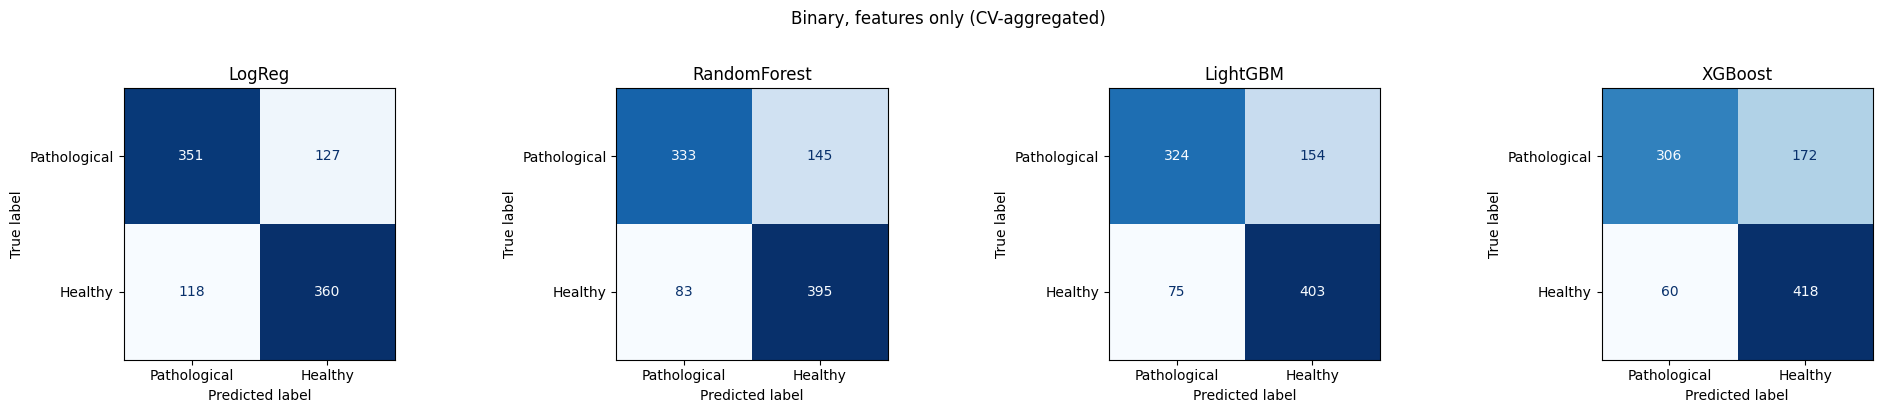
\includegraphics[width=\textwidth]{figures/binary_confusion_v8.png}
  \caption{Confusion matrices for binary classification with signal features only (main set, aggregated over the five folds), one panel per classifier.}
  \label{fig:binary_confmat_models}
  \end{figure}


  %--------------------------------------------------------------
  \subsection{Disease Group Classification}
  %--------------------------------------------------------------

Detecting pathology is one task. Sorting disorders by clinical cause is a harder one. The pathologies here are split into two clinical categories: neurological and structural.

Neurological disorders come from abnormal neural control of the vocal folds, structural disorders from abnormalities in the tissue of the folds themselves. Separating the two groups from the speech signal alone is difficult.

  Table~\ref{tab:multiclass_results} summarises the performance of the evaluated models for disease-group classification.

  \begin{table}[htbp]
  \centering
  \caption{Disease Group Classification Results (Mean $\pm$ SD over Five Folds)}
  \label{tab:multiclass_results}
  \begin{tabular}{llllc}
  \toprule
  \textbf{Inputs} & \textbf{Set} & \textbf{Best Model} & \textbf{Bal.\ Acc.} & \textbf{F1 Macro} \\
  \midrule
  Age only & Main & Random Forest & 0.553 & $0.536 \pm 0.069$ \\
  Sex only & Main & XGBoost & 0.606 & $0.605 \pm 0.091$ \\
  Age + sex & Main & XGBoost & 0.604 & $0.592 \pm 0.083$ \\
  Signal features & Main & XGBoost & 0.636 & $0.635 \pm 0.058$ \\
  Signal features + age + sex & Main & XGBoost & 0.652 & $\mathbf{0.649 \pm 0.066}$ \\
  \midrule
  Age + sex & Matched & LightGBM & 0.341 & $0.332 \pm 0.058$ \\
  Signal features & Matched & Random Forest & 0.580 & $\mathbf{0.575 \pm 0.042}$ \\
  \bottomrule
  \end{tabular}
  \end{table}

  Disease-group classification is much harder than binary pathology detection. Without demographic inputs the best model reaches 0.635 macro F1, and adding age and sex raises this only to 0.649, so age plays a smaller part here than in the binary task; the two groups differ by seven years on average (57.0 vs.\ 49.9). On the matched subset the score falls to 0.575, although this subset is also 42\% smaller than the full one. The acoustic differences between neurological and structural disorders are far less clear-cut than those between healthy and pathological voices.

  Figure~\ref{fig:multiclass_confusion} shows the confusion matrices for this task.

  \begin{figure}[htbp]
  \centering
  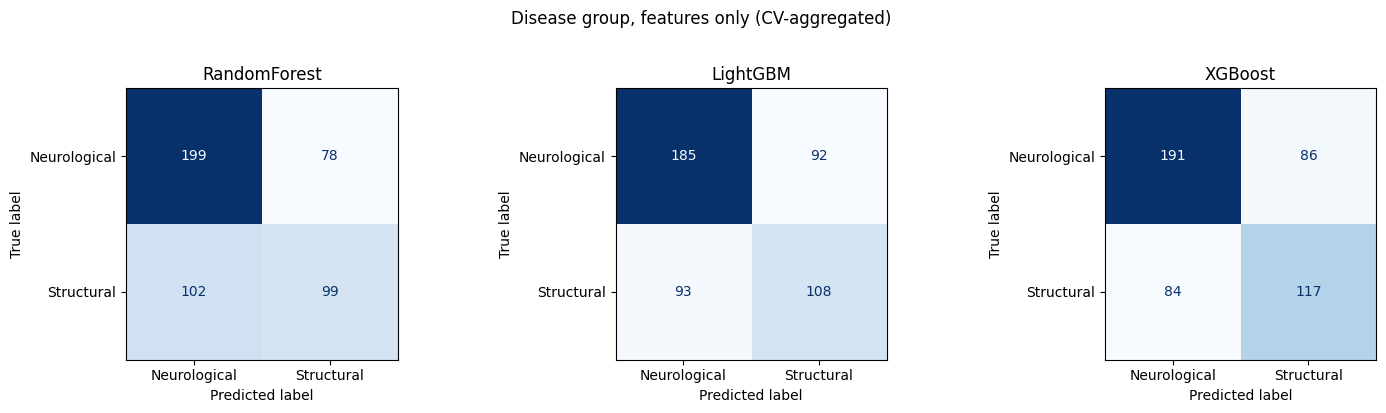
\includegraphics[width=0.8\textwidth]{figures/multiclass_confusion_v8.png}
  \caption{Confusion matrices for disease-group classification with signal features only (aggregated over the five folds), one panel per classifier.}
  \label{fig:multiclass_confusion}
  \end{figure}

  %--------------------------------------------------------------
  \subsection{Feature Ablation Analysis}
  %--------------------------------------------------------------

  A feature ablation study measures what each feature family contributes. We evaluated every combination of multifractal, OpenSMILE, and NeuroKit2 features under the same speaker-grouped protocol: without demographic inputs on the main set and the matched subsets, and with age and sex added on the main set. Table~\ref{tab:ablation_binary} lists the results together with the demographic baselines.

  \begin{table}[htbp]
  \centering
  \caption{Feature Ablation (Macro F1, Mean $\pm$ SD over Five Folds, Best Classifier per Cell). Signal features are used without age and sex except in the ``+\,age, sex'' column.}
  \label{tab:ablation_binary}
  \setlength{\tabcolsep}{6pt}
  \resizebox{\textwidth}{!}{%
  \begin{tabular}{lccccc}
  \toprule
  & \multicolumn{3}{c}{\textbf{Binary}} & \multicolumn{2}{c}{\textbf{Disease group}} \\
  \cmidrule(lr){2-4}\cmidrule(lr){5-6}
  \textbf{Features} & \textbf{Main} & \textbf{Main\,+\,age, sex} & \textbf{Matched} & \textbf{Main} & \textbf{Matched} \\
  \midrule
  MFDFA & $0.644 \pm 0.027$ & $0.854 \pm 0.015$ & $0.612 \pm 0.028$ & $0.560 \pm 0.079$ & $0.540 \pm 0.115$ \\
  OpenSMILE & $0.765 \pm 0.036$ & $0.884 \pm 0.024$ & $0.662 \pm 0.063$ & $0.624 \pm 0.067$ & $0.580 \pm 0.040$ \\
  NeuroKit2 & $0.687 \pm 0.036$ & -- & $0.610 \pm 0.051$ & $0.559 \pm 0.059$ & $0.585 \pm 0.084$ \\
  MFDFA + OpenSMILE & $0.766 \pm 0.039$ & $0.882 \pm 0.028$ & $0.664 \pm 0.022$ & $0.621 \pm 0.080$ & $0.587 \pm 0.046$ \\
  MFDFA + NeuroKit2 & $0.691 \pm 0.027$ & $0.868 \pm 0.031$ & $0.627 \pm 0.041$ & $0.566 \pm 0.091$ & $0.562 \pm 0.061$ \\
  OpenSMILE + NeuroKit2 & $0.767 \pm 0.051$ & $0.882 \pm 0.025$ & $0.668 \pm 0.049$ & $0.626 \pm 0.078$ & $0.591 \pm 0.046$ \\
  All three & $0.760 \pm 0.042$ & $0.882 \pm 0.025$ & $0.679 \pm 0.044$ & $0.635 \pm 0.058$ & $0.575 \pm 0.042$ \\
  \midrule
  Age only & $0.830 \pm 0.072$ & & $0.451 \pm 0.040$ & $0.536 \pm 0.069$ & $0.420 \pm 0.066$ \\
  Sex only & $0.532 \pm 0.055$ & & $0.435 \pm 0.065$ & $0.605 \pm 0.091$ & $0.429 \pm 0.052$ \\
  Age + sex & $0.846 \pm 0.017$ & & $0.386 \pm 0.061$ & $0.592 \pm 0.083$ & $0.332 \pm 0.058$ \\
  \bottomrule
  \end{tabular}}
  \end{table}

  \begin{figure}[htbp]
  \centering
  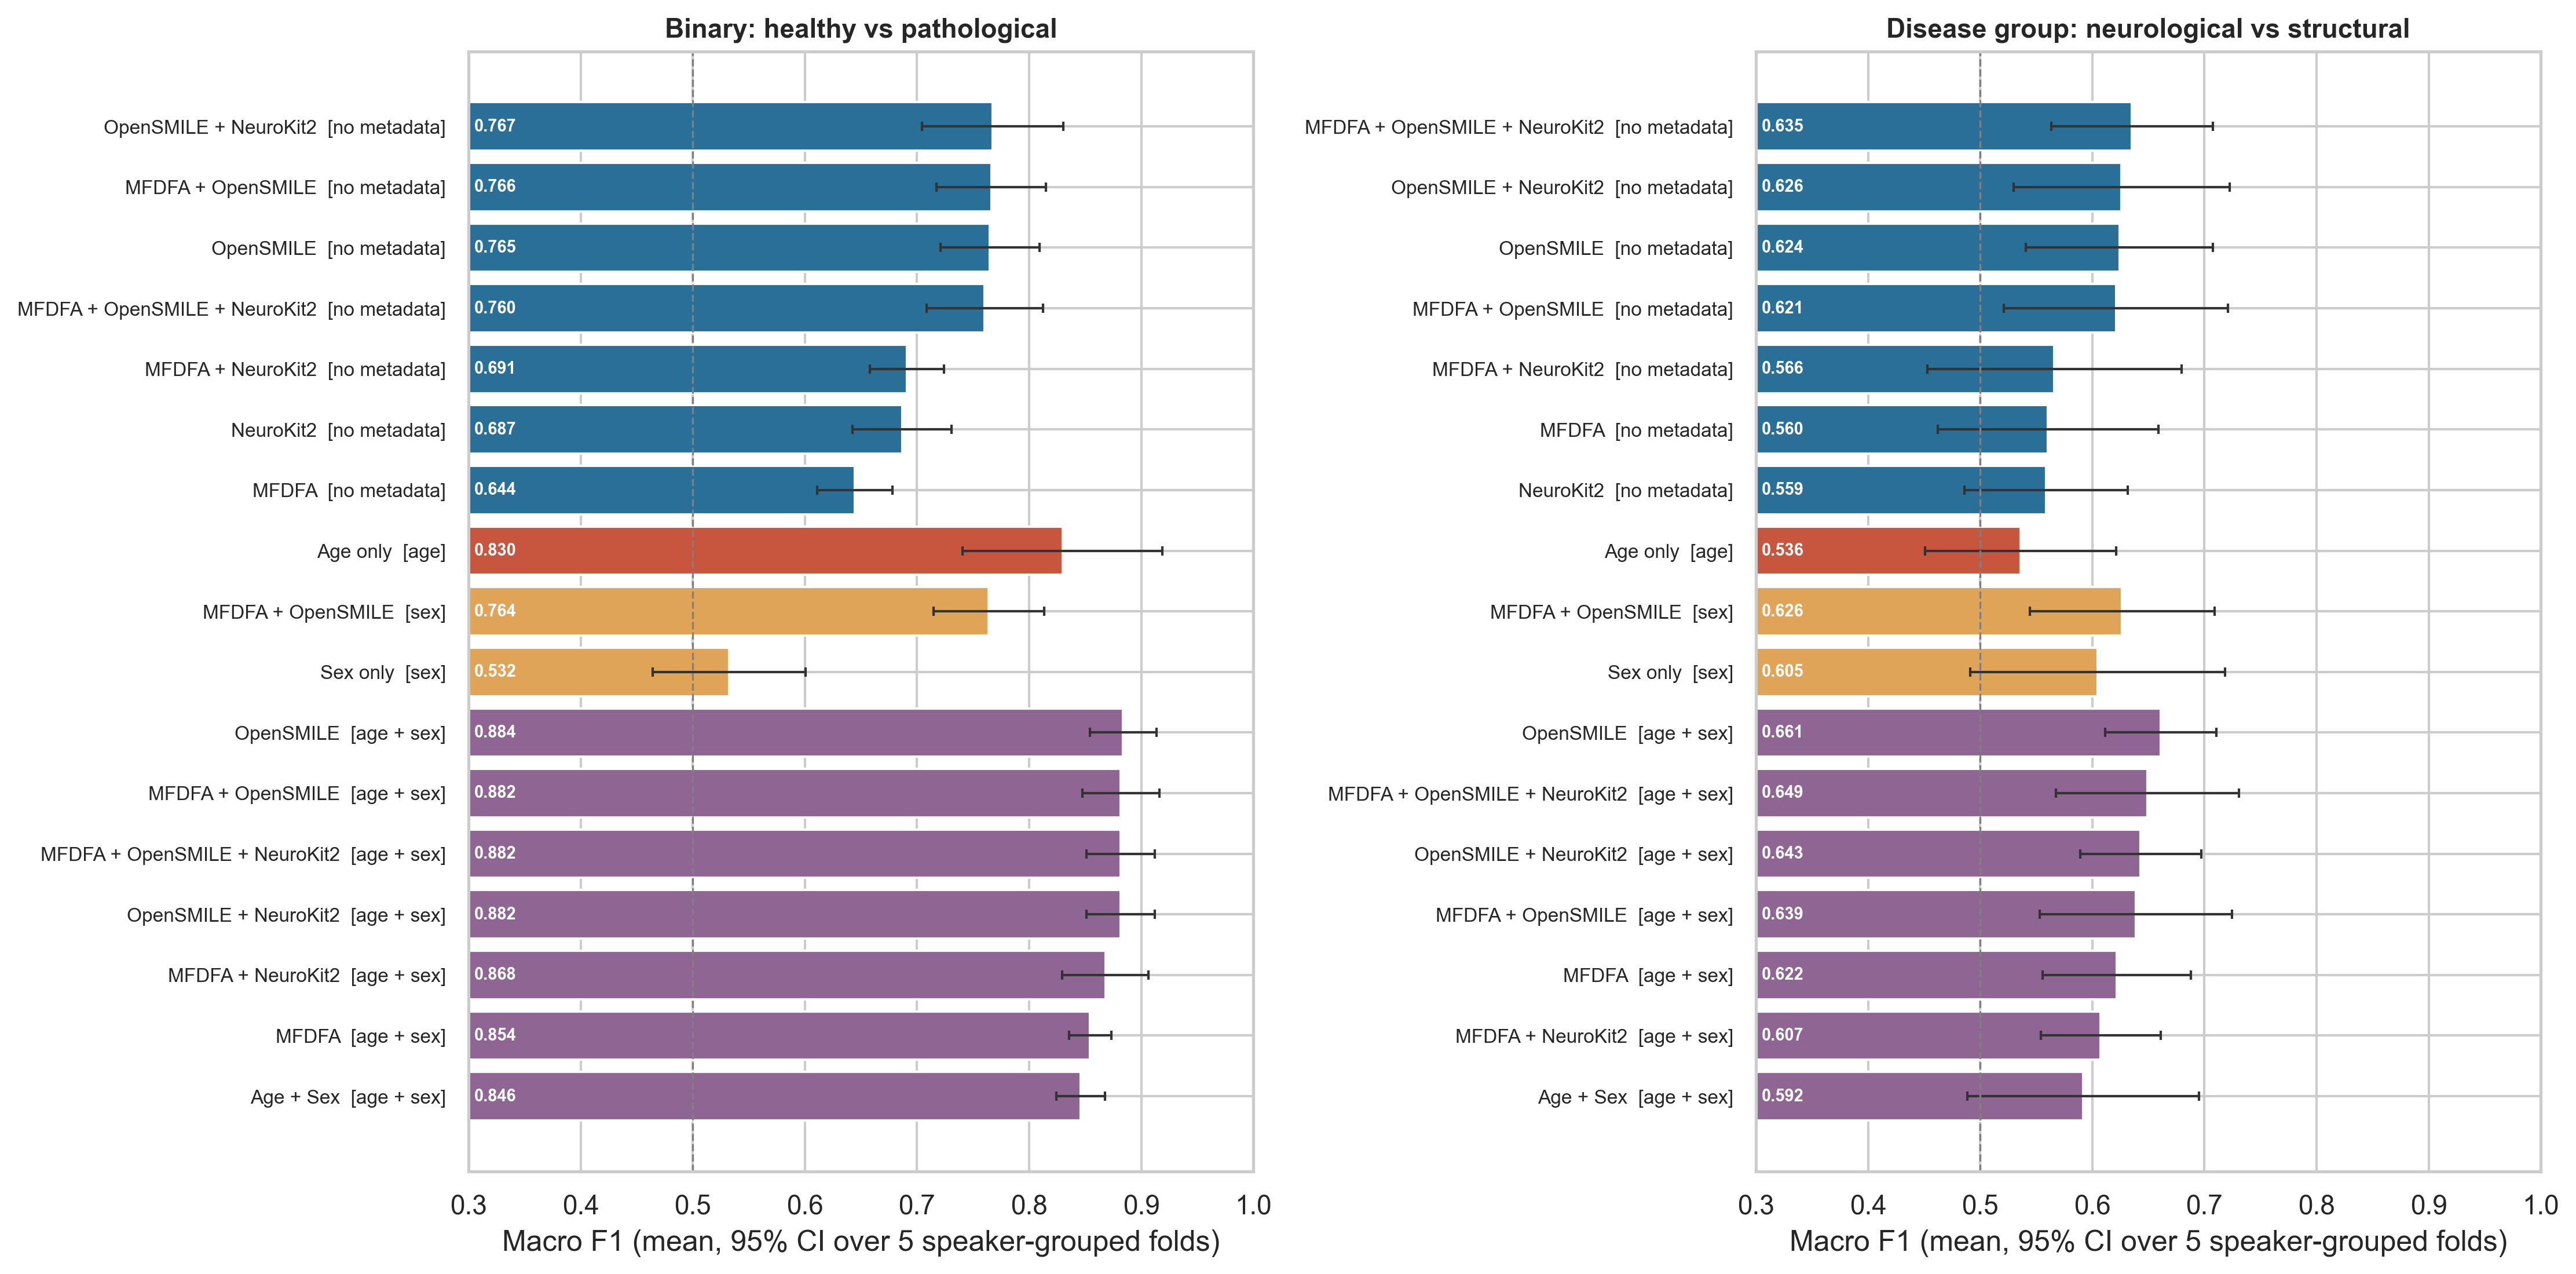
\includegraphics[width=0.68\textwidth,trim={0 0 533.8 0},clip]{figures/feature_ablation_v2.png}\\[1.5ex]
  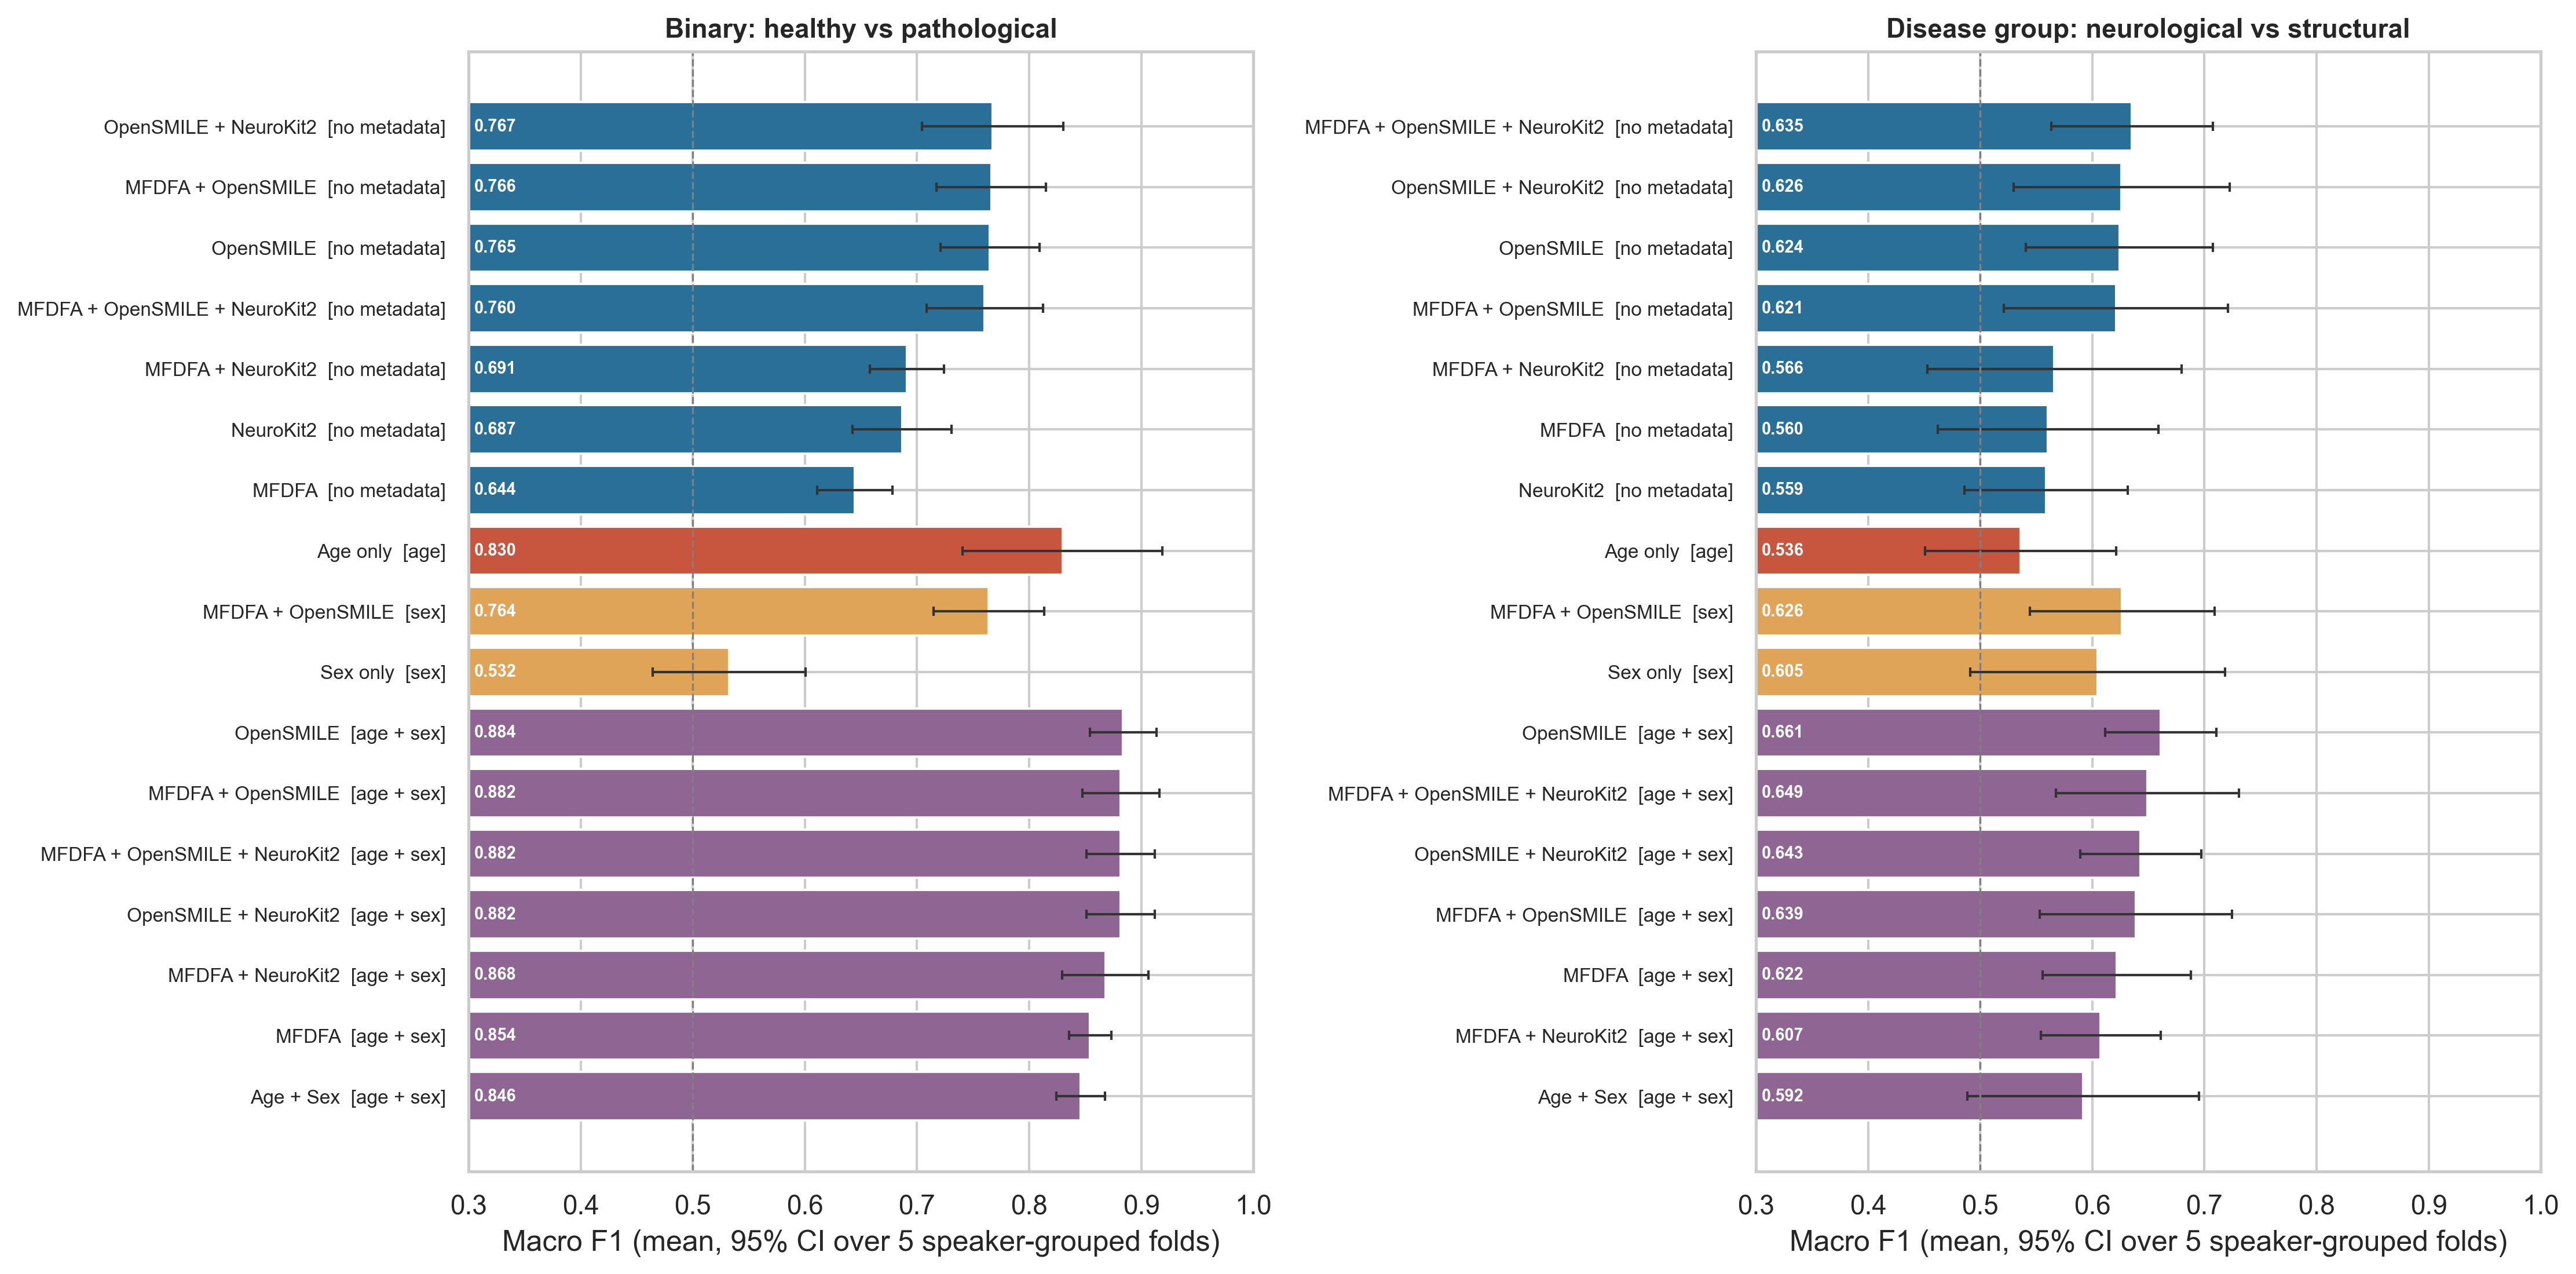
\includegraphics[width=0.68\textwidth,trim={533.8 0 0 0},clip]{figures/feature_ablation_v2.png}
  \caption{Feature ablation on the main set with 95\% confidence intervals over the five folds. Bar colour marks the demographic inputs used.}
  \label{fig:ablation_results}
  \end{figure}

On their own, the MFDFA descriptors reach 0.644 macro F1 on the binary task and 0.612 on the matched subset, so the scaling behaviour of the voice does carry information about pathology. OpenSMILE carries more: 0.765 on the main set and 0.662 on matched data. Combining the two gives 0.766 and 0.664, and removing MFDFA from the full feature set changes the score by less than 0.02 in every setting, well within the variation between folds. The picture is the same for disease groups, where MFDFA alone reaches 0.560 and adds nothing to OpenSMILE. The standard parameters already capture most of what MFDFA measures. NeuroKit2 likewise adds little once OpenSMILE is present.

Age dominates every configuration that includes it. Adding age and sex to any set of signal features raises the binary score to between 0.854 and 0.884, close to the 0.846 that age and sex reach alone, and the demographic baselines fall to chance on the matched subsets. Figure~\ref{fig:ablation_results} compares all configurations on the main set.

  %--------------------------------------------------------------
  \subsection{Per-Disease Binary Detection}
  %--------------------------------------------------------------

  A separate binary classifier was trained for each disease with at least ten recordings against an equal number of healthy recordings, to see which pathologies are individually detectable. Three settings are compared: all signal features with age and sex, the signal features alone, and the signal features on a subset in which each diseased recording is matched to a healthy one of the same sex within two years of age. The matched result is omitted when fewer than 20 pairs are found.

  \begin{table}[htbp]
  \centering
  \caption{Per-Disease Binary Detection (Macro F1, Mean $\pm$ SD over Five Folds, Best Classifier per Cell)}
  \label{tab:per_disease}
  \setlength{\tabcolsep}{6pt}
  \resizebox{\textwidth}{!}{%
  \begin{tabular}{l c c c c}
  \toprule
  \textbf{Disease} & \textbf{n} & \textbf{Features\,+\,age, sex} & \textbf{Features only} & \textbf{Matched (pairs)} \\
  \midrule
  Recurrent laryngeal nerve paralysis & 212 & $0.882 \pm 0.028$ & $0.786 \pm 0.032$ & $0.696 \pm 0.085$ (85) \\
  Reinke's edema & 67 & $0.828 \pm 0.062$ & $0.777 \pm 0.056$ & $0.742 \pm 0.051$ (45) \\
  Psychogenic dysphonia & 88 & $0.806 \pm 0.072$ & $0.714 \pm 0.140$ & $0.633 \pm 0.116$ (59) \\
  Laryngitis & 140 & $0.772 \pm 0.040$ & $0.683 \pm 0.065$ & $0.601 \pm 0.119$ (99) \\
  Functional dysphonia & 107 & $0.766 \pm 0.044$ & $0.610 \pm 0.052$ & $0.562 \pm 0.087$ (85) \\
  Vocal fold polyp & 44 & $0.754 \pm 0.141$ & $0.683 \pm 0.068$ & $0.544 \pm 0.164$ (36) \\
  Hyperfunctional dysphonia & 205 & $0.753 \pm 0.067$ & $0.657 \pm 0.030$ & $0.602 \pm 0.080$ (132) \\
  Spasmodic dysphonia & 64 & $0.699 \pm 0.184$ & $0.663 \pm 0.226$ & $0.713 \pm 0.227$ (25) \\
  Vocal fold nodules & 17 & $0.683 \pm 0.169$ & $0.683 \pm 0.169$ & -- (16) \\
  \bottomrule
  \end{tabular}}
  \end{table}

  Every disease except spasmodic dysphonia and vocal fold nodules loses accuracy once age is removed from the inputs or controlled by matching. Reinke's edema (0.742) and recurrent laryngeal nerve paralysis (0.696) remain clearly detectable on matched data, while vocal fold polyp (0.544) and functional dysphonia (0.562) fall close to chance. The spasmodic dysphonia estimate rests on only 12 speakers and varies widely between folds. Vocal fold nodules could not be matched in sufficient number, but their patients are young (34.4 years on average), so age plays little part in their unmatched score. Detecting individual disorders from a sustained vowel is harder than the unmatched scores suggest.


  %--------------------------------------------------------------
  \section{Conclusion}
  \label{sec:conclusion}
  %--------------------------------------------------------------

  This paper investigates multifractal descriptors obtained via MFDFA for automated voice pathology detection on the Saarbrücken Voice Database. MFDFA features are combined with conventional acoustic (OpenSMILE) and complexity-based (NeuroKit2) descriptors and evaluated under strict speaker-independent cross-validation, so the reported scores apply to unseen speakers.

  With age and sex among the inputs, binary pathology detection reaches a macro F1 of 0.882, but most of this reflects the age gap between healthy and pathological speakers in the Saarbr\"ucken Voice Database: age alone reaches 0.830. With age and sex controlled by matching, the signal features still detect pathology at 0.679, and disease-group classification reaches 0.575. The MFDFA descriptors carry information on their own (0.644 on the binary task) but add nothing measurable once the OpenSMILE parameters are present. Per-disease detection drops for almost every disorder after matching. For now the method suits screening better than differential diagnosis, and results on this corpus should be read with its age imbalance in mind.

  The study has limitations. It uses a single sustained vowel, and the matched evaluation covers speakers of roughly 15 to 75 years, with few healthy speakers over 60.

  Next steps are validation on larger independent cohorts with age-balanced controls, extension to multiple tokens and to end-to-end models, and an analysis of which parts of the multifractal spectrum carry the clinically useful signal.

%--------------------------------------------------------------
% References -- Springer 'splncs04' style, generated by BibTeX from refs.bib.
% Build: pdflatex paper_ccis && bibtex paper_ccis && pdflatex paper_ccis (x2)
% splncs04.bst sorts alphabetically by first author, so reference numbers do
% NOT follow order of citation. That is correct for LNCS/CCIS.
% Ship paper_ccis.bbl alongside the source; Springer requires it.
%--------------------------------------------------------------
\bibliographystyle{splncs04}
\bibliography{refs}
\end{document}
